\documentclass{article}
\title{Blanchard Ch.9}
\author{Dawei Wang}
\date{\today}
\usepackage{ctex}
\usepackage{amsmath}
\usepackage{amssymb}
\usepackage{graphicx} %插入图片的宏包
\usepackage{float} %设置图片浮动位置的宏包
\usepackage{subfigure} %插入多图时用子图显示的宏包
\begin{document}
	\maketitle
\section{IS-LM-PC模型}

短期方程:

\[
Y=C(Y-T)+I(Y,r+x)+G
\]

\begin{figure}[H] %H为当前位置,!htb为忽略美学标准,htbp为浮动图形
	\centering %图片居中
	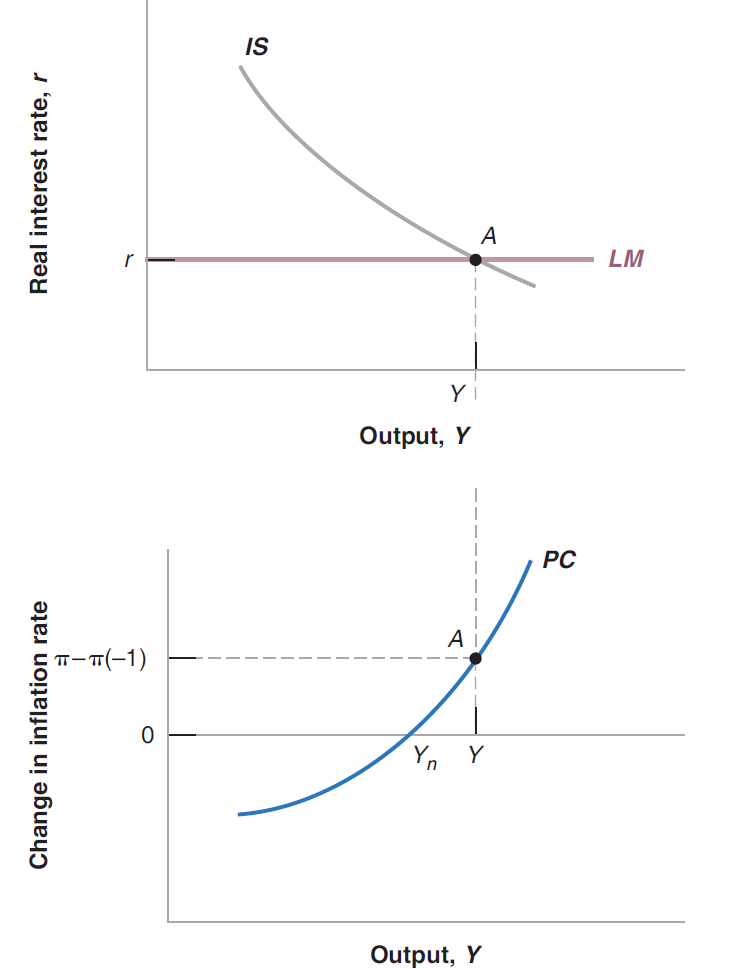
\includegraphics[width=1\textwidth]{9_1} %插入图片,[]中设置图片大小,{}中是图片文件名
	\caption{The IS-LM-PC Model} %最终文档中希望显示的图片标题
	\label{Fig.main2} %用于文内引用的标签
\end{figure}

菲利普斯曲线:

\[
\pi-\pi^e=-\alpha(u-u_n)
\]

\hspace*{\fill}

从产出的角度重写菲利普斯曲线:

根据定义:

\[
u\equiv U/L=(L-N)/L=1-N/L
\]

变化得:

\[
N=L(1-u)
\]

假设就业等于产出:

\[
Y=N=L(1-u)
\]

当失业率等于自然失业率$ u_n $时,就业给定等于$ N_n=L(1-u_n) $,产出等于$ Y_n=L(1-u_n) $。$ N_n $称为自然就业水平,$ Y_n $称为自然产出水平,也被称为潜在输出(potential output)。

因此可以将就业偏离其自然水平表述为:

\[
Y-Y_n=-L(u-u_n)
\]

产出与潜在产出之间的差值称为产出缺口(output gap),这个等式与产出和失业之间的实际关系,称为奥肯定律。

将$ u-u_n $替换,得到新的菲利普斯曲线:

\[
\pi-\pi^e=\frac{\alpha}{L}(Y-Y_n)
\]

假设预期今年的通货膨胀率等于去年的通胀率:

\[
\pi-\pi(-1)=\frac{\alpha}{L}(Y-Y_n)
\]

当产出高于潜在水平产出缺口为正,通货膨胀增加,反之反是。因此菲利普斯曲线与横轴的交叉点即为产出处在潜在水平的位置。

\subsection{跨时间与国度的奥肯定律}

失业与产出之间的关系:

\[
u-u(-1)\approx -g_Y
\]

推导:

就业、劳动力和失业率之间的关系

\[
N=L(1-u)
\]

上一年度的关系

\[
N(-1)=L(1-u(-1))
\]

二者结合

\[
N-N(-1)=L(1-u)-L[1-u(-1)]=-L[u-u(-1)]
\]

两边同除以N(-1),得到:

\[
\frac{N-N(-1)}{N(-1)}=-\frac{L}{N(-1)}[u-u(-1)]
\]

假设就业等于产出,则就业增长率等于产出增长率,还应注意$ L/N(-1) $近似等于1。

因此

\[
u-u(-1)\approx -g_Y
\]

\hspace*{\fill}

实际上上每年的产出增长率要大于一定值,以防止失业率上升。这时因为我们在推导过程中忽略了两个因素:劳动力的增长和劳动生产率的增长。要保持恒定的失业率,就业必须以劳动力相同的速度增长。仅仅为了保持恒定的失业率,产出就必须等于劳动力增长和劳动生产率增长的总和。

另外,当产出增长率高于正常水平的1\%,失业率的降低少于1\%。

原因一:无论产出水平如何,一些工人的需求一定。

原因二:劳动力囤积——由于培训成本企业在经济不景气时不解雇员工,当产量高于正常水平的时候,公司要求他们加班而不是招聘新员工。

\hspace*{\fill}

就业率的提高不会导致失业率一对一下降:

原因是劳动力参与率的增加。当就业率增加时,并不是所有新工作都由失业者填补。有些工作是给那些被归类为劳动力以外的人员做的,这意味着他们没有积极地寻找工作,此外,一些先前被列为劳动力以外的气馁的工人决定积极寻找工作,并被列为失业者。

由于这两个原因,失业率下降少于就业增加。

因此,失业对就业变动的反应少于1,而就业变动本身对产出反应小于1。

定义奥肯系数(Okun coefficient)为产出增长对失业率变动的影响。这个系数因国家而异。

\section{动态调整与中期调整}

\begin{figure}[H] %H为当前位置,!htb为忽略美学标准,htbp为浮动图形
	\centering %图片居中
	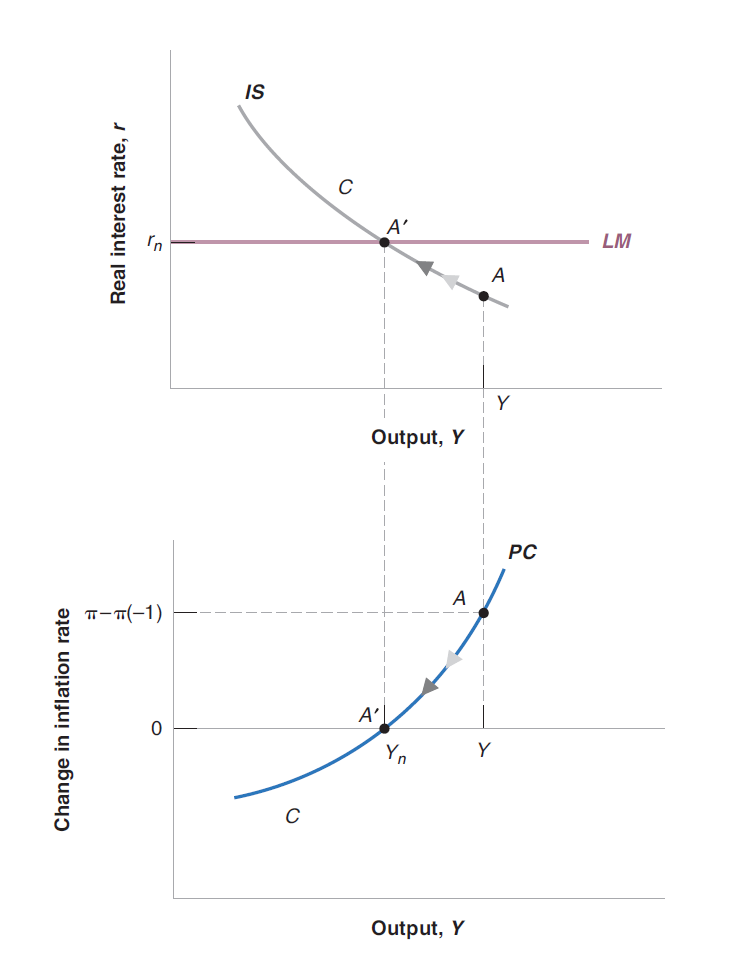
\includegraphics[width=1\textwidth]{9_2} %插入图片,[]中设置图片大小,{}中是图片文件名
	\caption{Medium-Run Output and
		Inflation} %最终文档中希望显示的图片标题
	\label{Fig.main3} %用于文内引用的标签
\end{figure}

当产出位于Y,从下图可以看出,Y高于潜在水平$ Y_n $,这意味着通货膨胀正在增加。非正式地说,经济过热给通货膨胀带来压力。这是短期均衡。

如果政策利率或任何影响IS曲线位置的变量均没有变化,随着时间推移产出仍然高于潜在水平,通货膨胀继续增加。然而,在某个时候,政策可能会对通货膨胀做出反应。把重点放在中央银行,中央银行迟早会提高政策利率,从而将产出降至潜在水平,不再对通货膨胀施加压力。经济会沿着IS曲线上升至$ A' $,在$ A' $点上,政策利率等于$ r_n $,产出等于$ Y_n $,这意味着通货膨胀恒定,这是中期均衡。与$ Y_n $相关联的利率$ r_n $通常为自然利率(natural rate of interest),有时也被称为中性利率(netural rate of interest),或维克塞尔利率(Wicksellian rate of interest)。

由于中央银行往往很难知道潜在产出的确切位置,进而知道产出距离潜在水平有多远。通货膨胀变化提供了一种产出缺口信号,但是该信号拥有太多噪声。因此,中央银行可能希望缓慢调整产政策利率,以观看会发生什么。其次,经济调整需要时间做出反应。

产出恢复到自然水平需要时间这一事实引起了通货膨胀问题,在调整过程中,产出始终高于潜在水平,因此通货膨胀不断增加。因此当经济达到$ A' $点时,通货膨胀率高于A点的位置。如果银行既关注通货膨胀稳定,也关注通货膨胀水平,那么它很可能决定不仅要稳定,还要降低通货膨胀。为此它需要将政策利率提高到$ r_n $以上,以降低通货膨胀,直到通货膨胀恢复到中央银行可接受的水平。

换句话说,如果中央银行希望在中期内实现恒定通货膨胀水平,那么衰退总是跟在最初的繁荣之后。

\subsection{重新审视预期的作用}

假设人们预期通货膨胀不是等于去年的通货膨胀$ \pi(-1) $,而是等于常数$ \overline{\pi} $。此时:

\[
\pi-\overline{\pi}=(\frac{\alpha}{L})(Y-Y_n)
\]

正的产出缺口会产生比预期更高的通货膨胀而非通货膨胀的增加。为了使通货膨胀恢复到$ \overline{\pi} $,在这种情况下,中央银行没有必要像以前那样在一段时间内提高利率到$ r_n $以上。因此,中央银行的工作更容易。只要通货膨胀预期锚定(anchored),它就不需要通过后来的衰退来弥补最初的繁荣。

\subsection{零利率下限与债务螺旋}

\begin{figure}[H] %H为当前位置,!htb为忽略美学标准,htbp为浮动图形
	\centering %图片居中
	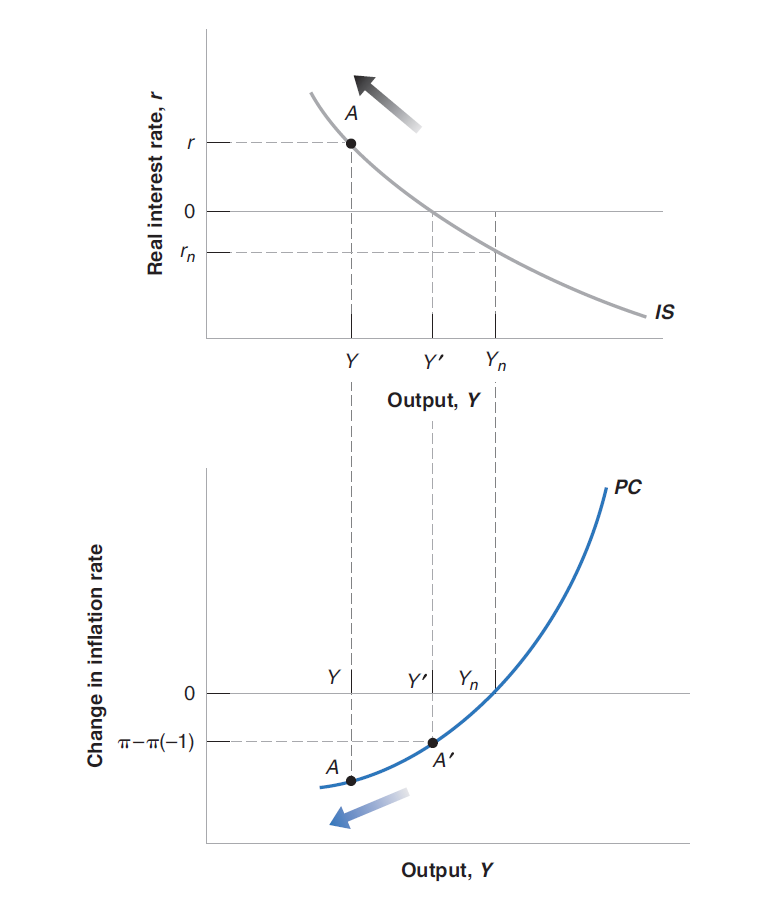
\includegraphics[width=1\textwidth]{9_3} %插入图片,[]中设置图片大小,{}中是图片文件名
	\caption{The Deflation Spiral} %最终文档中希望显示的图片标题
	\label{Fig.main4} %用于文内引用的标签
\end{figure}

考虑经济衰退的情况,目前政策利率为r,产出为Y,远低于$ Y_n $。产出缺口为负,通货膨胀不断下降,如果经济足够萧条,将产出恢复到自然水平所需的实际政策利率$ r_n $可能是负的。然而,零利率下限约束将使这种负的实际利率政策不可能实现。此时,即使中央银行将名义利率设为零,产出将仍低于潜在水平,因此通货膨胀仍在下降。这就开始了经济学家所说的通货紧缩螺旋(deflation spiral)或通货紧缩陷阱(deflation trap)。

继续假设工资设定者预期通货膨胀与去年相同,因此负的产出缺口意味着通货膨胀下降,如果通货膨胀一开始等于零,它就会变成负值。零通货膨胀变成通货紧缩。反过来,这意味着即使名义利率保持为零,实际政策利率越高,产出越低。此时经济不仅没有收敛到中期均衡位置,而是远离了均衡点,产出稳步下降,通货紧缩稳步扩大。中央银行无能为力,经济每况愈下。

\hspace*{\fill}

\section{重新审视财政整合}

\begin{figure}[H] %H为当前位置,!htb为忽略美学标准,htbp为浮动图形
	\centering %图片居中
	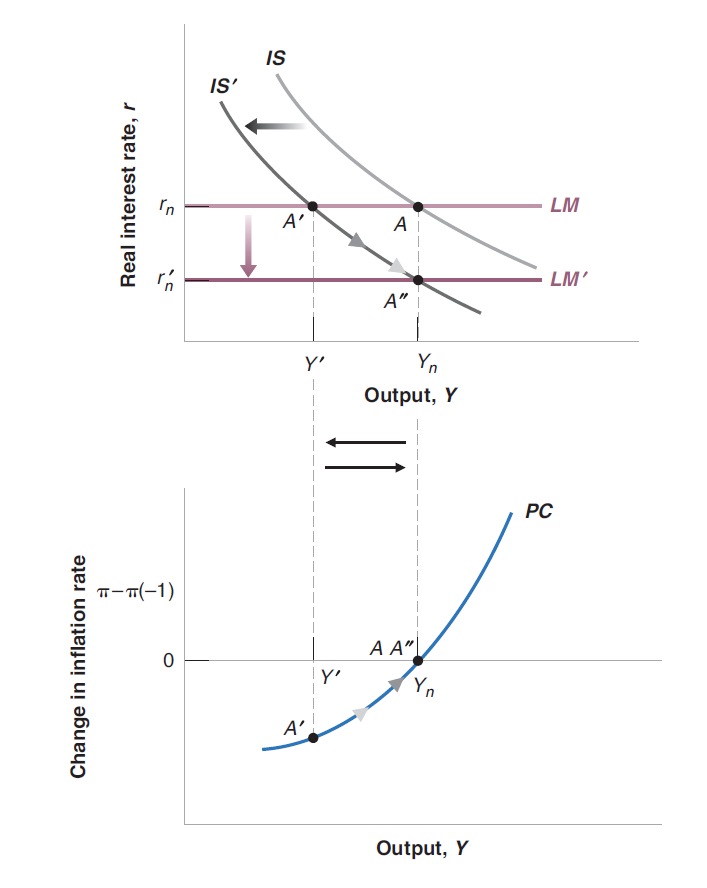
\includegraphics[width=1\textwidth]{9_4} %插入图片,[]中设置图片大小,{}中是图片文件名
	\caption{Fiscal Consolidation
		in the Short and the
		Medium Run} %最终文档中希望显示的图片标题
	\label{Fig.main5} %用于文内引用的标签
\end{figure}

假设政府加税,IS曲线左移至$ IS' $,新的短期均衡由$ A' $点给出。在给定政策利率$ r_n $下,产出从Y下降到$ Y' $,通货膨胀开始下降。随着收入下降和税收增加,消费都有所下降。同时随着产出减少,投资也在减少。

转向动态调整和中期均衡。由于产出太低,通货膨胀率不断下降,中央银行可能会做出反应,降低政策利率,直到产出恢复至潜在水平。此时新的均衡在$ A'' $,现在需要维持产出处在潜在水平的政策利率低于前值。

由于收入与财政整合前相同,但税率较高,因此消费较低,尽管没有短期低。由于产出与以前一样,但利率较低,因此投资高于以前。换句话说,消费的减少被投资的增加所抵消,因此需求和隐含的需求保持不变。虽然整合可能在短期内减少投资,但在中期会增加投资。看起来似乎可以采取财政整合,并且在短期内不会降低产出,所需要的是中央银行和政府认真协调。在进行财政整合时,中央银行应制定政策利率,以便使产出保持在自然水平。

\section{石油价格上涨的影响}

通过增加m——价格高于名义工资的溢价。给定工资,石油价格的上涨会增加生产成本,迫使企业提高价格以保持相同的利润率。作出这一假设后,我们就可以跟踪溢价增长对产出和通货膨胀的影响了。

\subsection{对自然失业率的影响}

\begin{figure}[H] %H为当前位置,!htb为忽略美学标准,htbp为浮动图形
	\centering %图片居中
	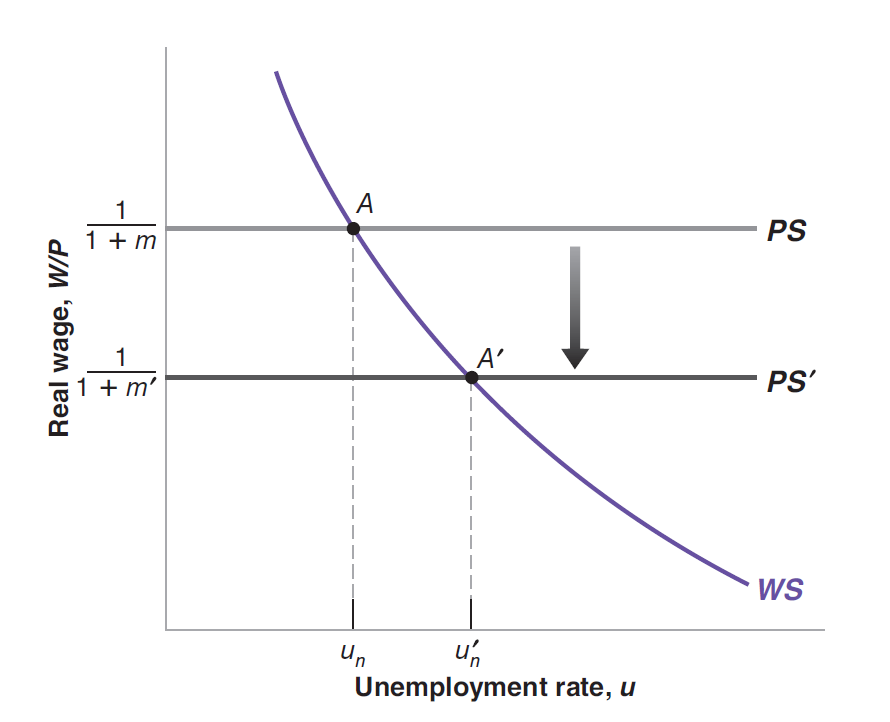
\includegraphics[width=1\textwidth]{9_5} %插入图片,[]中设置图片大小,{}中是图片文件名
	\caption{The Effects of an Increase
		in the Price of Oil on
		the Natural Rate of
		Unemployment} %最终文档中希望显示的图片标题
	\label{Fig.main6} %用于文内引用的标签
\end{figure}

初始均衡点在A点,初始自然失业率为$ u_n $。溢价越高,价格设定所隐含的实际工资就越低。均衡点从A移动到$ A' $。实际工资降低,自然失业率增加。公司因为必须为石油支付更多的成本,所以它们可以支付的工资更低,要使工人接受较低的实际工资,就需要增加失业率。如果我们假设就业和产出的关系不变,那么自然就业水平的下降就会导致潜在产出同样下降。

\begin{figure}[H] %H为当前位置,!htb为忽略美学标准,htbp为浮动图形
	\centering %图片居中
	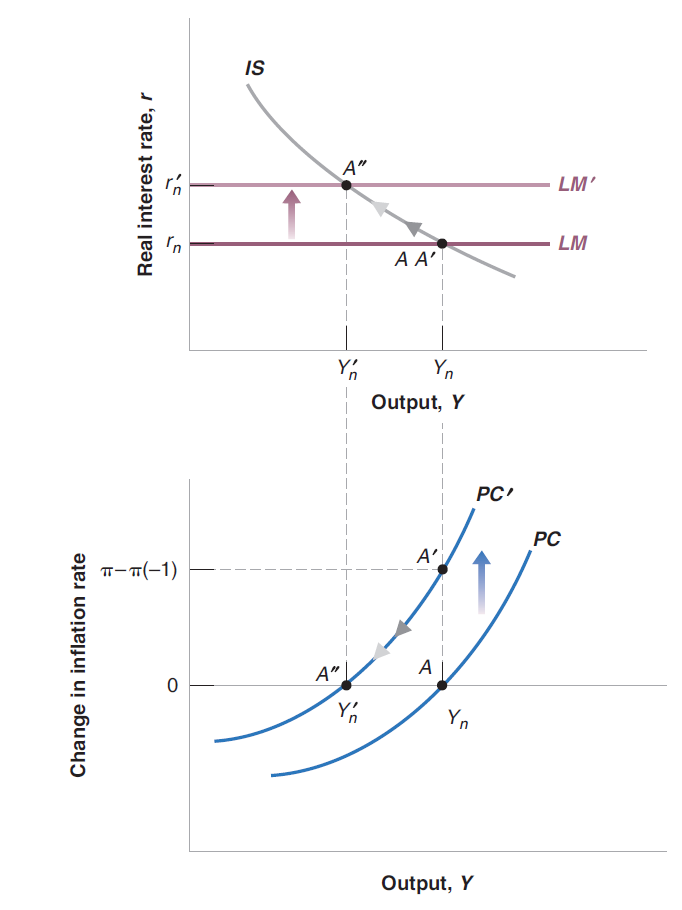
\includegraphics[width=1\textwidth]{9_6} %插入图片,[]中设置图片大小,{}中是图片文件名
	\caption{Short and Medium Run
		Effects of an Increase in
		the Price of Oil} %最终文档中希望显示的图片标题
	\label{Fig.main7} %用于文内引用的标签
\end{figure}

随着石油价格的增长,自然产出水平降低,也就是说从$ Y_n $变到$ Y_n' $。菲利普斯曲线向上移动,由pc移动到$ PC' $。如果IS曲线没有移动,而中央银行没有改变政策利率,产出不会改变,但同一水平的产出现在与较高的通货膨胀有关。从短期来看,产出没有变化,但通货膨胀率较高。

转向动态调整问题。如果中央银行保持政策利率不变,产出将继续超过现在较低的潜在产出水平,通货膨胀将继续上升,因此在某个时候,中央银行将提高政策利率以稳定通货膨胀。一旦经济处于$ A'' $点,经济就处于中期均衡状态。由于潜在产出较低,石油价格的上涨反映在永久低水平产出。较低的产出水平和较高的通货膨胀联系在一起,这个组合经济学家称为滞涨(stagflation)。

\hspace*{\fill}

P.S.:

第一个问题是我们假设IS曲线不会移动,事实上,石油价格上涨可能会通过多种渠道影响需求并改变IS曲线。因此IS曲线很有可能向左移动,不仅在中期内,而且在短期内也会导致产出下降。

第二个问题与通货膨胀的演变有关。当经济到达$ A'' $点时,通货膨胀率高于石油价格上涨前的水平,如果中央银行希望将通货膨胀率恢复到初始水平,就必须在一段时间内将产出降至潜在水平以下,以降低通货膨胀率。

第三个问题与第二个问题有关,如果不假设通胀等于去年的通胀,在这种情况下,高于潜在水平的产出将导致高通货膨胀,而不仅仅增加通货膨胀。然后随着产出下降到较低的潜在水平,通胀也下降了。当经济到达$ A'' $点时,通货膨胀又回到石油价格上涨之前的水平。中央银行没必要进一步减少产出,以降低通货膨胀。

\section{结论}

\subsection{短期运行与中期运行}

冲击或政策变化通常在短期和中期产生不同的影响。如果认为产出恢复到潜在水平需要很长时间,那么会更多地关注短期,并愿意采用短期内增加产出的政策,即使中期效应为零或负。相反,如果相信产出很快会恢复到潜在水平,那么将更重视中期影响,并因此更不愿意使用这些政策。


\subsection{冲击和传播机制}

经济不断受到冲击(shocks),每次冲击都会对产出及其构成产生动态影响。这些动态影响可能随着时间的推移而增加,从而影响中期均衡产出。或者这种影响可能会持续一段时间,然后逐渐减少并消失。













	
\end{document}